\chapter{Geometry Part II}

\subsection{SAT Worksheet 1B: Warm-Up Problems}

\textbf{Strategies Practice:} Read the question, then make a box around what you are trying to solve for. This may be different than what you are solving for, so it is a good check.

\begin{multienumerate}
\mitemxx{\basic

In square $ABCD$, $\angle A$ is $(1/3)x$. What is $(5/3)x$ equal to?

\begin{enumerate}[label=(\Alph*)]
\item $90^\circ$
\item $360^\circ$
\item $180^\circ$
\item $270^\circ$
\item $450^\circ$
\end{enumerate}
}{\medium

What is the measure, in degrees, of the largest of 3 angles that together form a straight line if the ratio of the angles is $5:4:1$?

\begin{enumerate}[label=(\Alph*)]
\item $18^\circ$
\item $72^\circ$
\item $80^\circ$
\item $90^\circ$
\item $180^\circ$
\end{enumerate}}
\end{multienumerate}

\hrulefill

\textbf{Content Practice:} Do the following problems.

\begin{multienumerate}
\mitemxx{\basic

In the $xy$-plane, the line with equation $y=4/5x+3$ intersects the $x$-axis at point $A$ and the $y$-axis at point $B$. What is the length of a line segment from point $A$ to point $B$ rounded to the nearest tenth?}
{\medium
If it is 4:00pm, what is the measure of the angle between the minute and hour hands of the clock?

\begin{enumerate}[label=(\Alph*)]
\item $30^\circ$
\item $90^\circ$
\item $120^\circ$
\item $160^\circ$
\item $180^\circ$
\end{enumerate}}

\mitemx{\advanced

Line $l$ has the equation $y=-6x+5$. What is the equation of line $l$ reflected over the $x$-axis?

\begin{enumerate}[label=(\Alph*)]
\item $-1/6x+5$
\item $6x+5$
\item $-1/6x-5$
\item $1/6x+5$
\item $6x-5$
\end{enumerate}
}
\end{multienumerate}

\newpage
\section{Circles}

Examples:

\begin{multienumerate}
\mitemxx{\basic

In an $xy$-plane, one endpoint of a diameter of a circle is $(-5,-6)$ and the other endpoint of the diamtere is $(7,-6)$. What is the center of the circle?

\begin{enumerate}[label=(\Alph*)]
\item $(0,0)$
\item $(12,-6)$
\item $(1,-6)$
\item $(1,6)$
\item $(12,-12)$
\end{enumerate}}{\medium

The diameter of circle $A$ is 4 times the diameter of circle $B$. What is the ratio of the area of circle $A$ to the area of circle $B$?

\begin{enumerate}[label=(\Alph*)]
\item 2
\item 4
\item 8
\item 12
\item 16
\end{enumerate}}
\end{multienumerate}

\bigskip
Review Questions:

\begin{enumerate}
\item What is the relationship between radius and diameter?
\vfill\item What is the formula for the circumference of a circle? For the circumference of a semicircle?
\vfill\item What is the formula for the area of a circle? Fro the area of a semicircle?
\vfill\item Many SAT problems with circles will give you the area of a circle and ask you to find the circumference of it OR give you the circumference of the circle and ask you to find the circle's area? Conceptually, how would you do either of these scenarios?
\end{enumerate}

\vfill
\newpage
\textbf{New Material}

\bigskip
What is a sector?

\hfill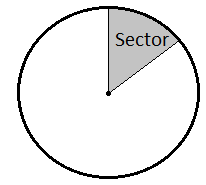
\includegraphics{16}

How can we compare the features of a sector (e.g. area) to the features of a circle and solve for the unknown features?

\vfill
What is the mathematical expression that will allow us to compare the features and solve for the unknown features?

\vfill
Demonstrate your knowledge of the concept by solving the problem below:

\bigskip
The area of circle $A$ (shown to the right) is $25\pi$ cm$^2$. If the area of sector $ABC$ is $10\pi$ cm$^2$, what is the length of arc $BC$?

\hfill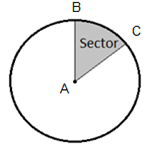
\includegraphics{17}

\newpage
\subsection{SAT Worksheet 2B: 6 Questions, 8 Minutes}

\begin{multienumerate}
\mitemxx{\basic

\centerline{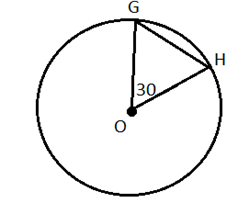
\includegraphics{18}}

\centerline{Note: Figure not drawn to scale}

\bigskip
In the figure above, point $O$ is the center of the circle and $\angle GOH = 30^\circ$. Given that each triangle must have one vertex touching $O$ and the triangles can not overlap, how many triangles identical to $GOH$ could be fit in circle $O$?

\begin{enumerate}[label=(\Alph*)]
\item 5
\item 6
\item 12
\item 24
\item 36
\end{enumerate}}{\basic

Three semicircles with radius 3 are placed on a rectangular sheet of paper with length 10 and width 15. None of the semicircles overlap and they are all completely on the paper. What is the area of the paper not covered by semicircles?

\begin{enumerate}[label=(\Alph*)]
\item $150-(27/2)\pi$
\item $150-(150/2)\pi$
\item $150-(9/2)\pi$
\item $150-(35/2)\pi$
\item $9/2\pi$
\end{enumerate}}

\vfill
\mitemxx{\medium

Joe cut 2 circular pizzas into identical wedge-shaped pieces. The tip of each piece is always at the center of the pizza and the angle at the tip is always greater than $30^\circ$ but smaller than $40^\circ$. Name one possible value for the number of total pieces into which the two pizzas are cut.
}{\medium

A circle has its center at $(2,3)$ and a radius of 4. Which of the following are $x$-coordinates on the circle that have the same $y$-coordinates?

\begin{enumerate}[label=(\Alph*)]
\item $(-1,5)$
\item $(2,3)$
\item $(6,0)$
\item $(-3,7)$
\item $(-2,3)$
\end{enumerate}}

\vfill
\mitemxx{\advanced

\centerline{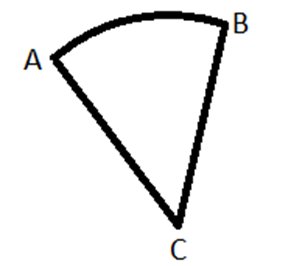
\includegraphics{19}}

In the figure above, $AB$ is the arc of a circle with center $C$. $\angle ACB$ is $40^\circ$. If the area of the circle C is $25\pi$, what is the length of arc $AB$?

\begin{enumerate}[label=(\Alph*)]
\item $2.5\pi$
\item $4.0\pi$
\item $(6/5)\pi$
\item $(10/9)\pi$
\item $1.3\pi$
\end{enumerate}
}{\advanced

\centerline{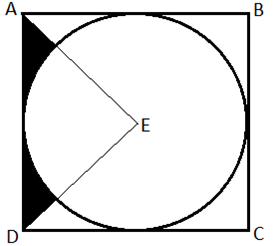
\includegraphics{20}}

In the figure above, square $ABCD$ has an edge of 6. What is the area of the shaded region?

\begin{enumerate}[label=(\Alph*)]
\item $9-(9/4)\pi$
\item $36-9\pi$
\item $36-(9/4)\pi$
\item $36-(9/16)\pi$
\item $9-(9/16)\pi$
\end{enumerate}}
\end{multienumerate}

\newpage
\section{Unusual and Multiple Figures}

Examples:

\begin{multienumerate}
\mitemxx{\medium

A cylinder with height $h$ and radius $e$ is stacked on top of a cube with an edge $e$. What is the ratio of the cylinder volume to the cube volume in terms of $h$ and $e$ in its most simplified form?

\begin{enumerate}[label=(\Alph*)]
\item $e^2h\pi$
\item $(e^2h/e^3)\pi$
\item $(h/e)\pi$
\item $e^{-2}h\pi$
\item $(e/h)\pi$
\end{enumerate}
}{\medium

\centerline{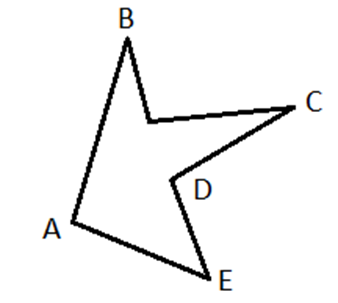
\includegraphics{21}}

In the figure above, the area is 39 square units and the perimeter is four less than two thirds of the area. If the ratio of $AB:BC:CD:DE:AE=3:1:2:2:1:2$, then what is the length of $AB$?

\begin{enumerate}[label=(\Alph*)]
\item 3
\item 4
\item 6
\item 9
\item 12
\end{enumerate}}
\end{multienumerate}

\hrulefill

Strategy for Unusual or Multiple Figures

\begin{enumerate}
\item
\item
\item
\item
\end{enumerate}

\pagebreak
\subsection{SAT Worksheet 3B: 6 Questions, 8 Minutes}

\begin{multienumerate}
\mitemxx{\basic

A plot of land has a perimeter of 48 square meters. What is the largest possible area for this plot of land, in square meters?

\begin{enumerate}[label=(\Alph*)]
\item 36
\item 48
\item 128
\item 144
\item 216
\end{enumerate}
}{\basic

Shape A consists of 22 identically shaped, small squares and has a perimeter of 24 meters and an area of 12 square meters. Shape B consists of 11 identically shaped, small squares that are the same size as the squares in Shape A and a perimeter of 15 meters. What is the area of Shape B, in square meters?

\begin{enumerate}[label=(\Alph*)]
\item 6
\item 7.5
\item 10
\item 11
\item 22
\end{enumerate}}

\vfill
\mitemxx{\medium

\centerline{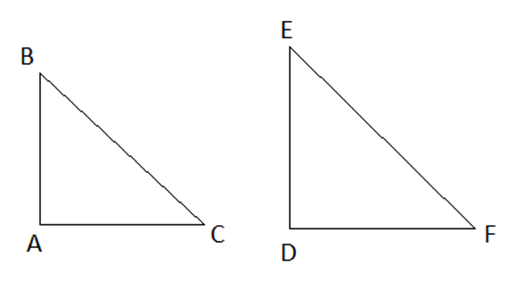
\includegraphics{22}}

Note: Figures are not drawn to scale

\bigskip
Triangles $ABC$ and $DEF$ are similar with a ratio of $5:6$. If $BA=10$, $\angle A$ is $90^\circ$ and $\angle B$ is $45^\circ$, what is the perimeter of triangle $DEF$?

\begin{enumerate}[label=(\Alph*)]
\item $20+10\sqrt2$
\item 30
\item $20+12\sqrt{2}$
\item $24+12\sqrt{2}$
\item 36
\end{enumerate}}
{\medium

\centerline{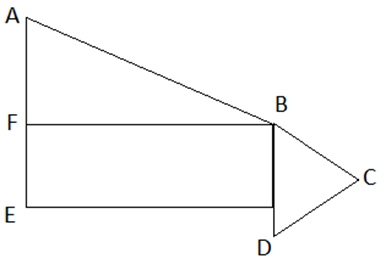
\includegraphics[scale=0.8]{23}}

Note: Figure is not drawn to scale

\bigskip
In the figure above, $BF\perp AF$ and $AF=FE=3$. $BD$ is twice as long as $AF$. If $\angle A=\angle C=\angle D=60^\circ$, what is the perimeter of the figure $ABCDEF$? (Note: The answer should include the perimeter of the unmarked vertex (where $BD$ and $E$ intersect), not just a straight line from $D$ to $E$.)

\begin{multicols}{2}
\begin{enumerate}[label=(\Alph*)]
\item $24+3\sqrt3$
\item 24
\item $20+3\sqrt2$
\item $20+3\sqrt3$
\item $20-3\sqrt3$
\end{enumerate}
\end{multicols}}

\vfill
\mitemxx{\advanced

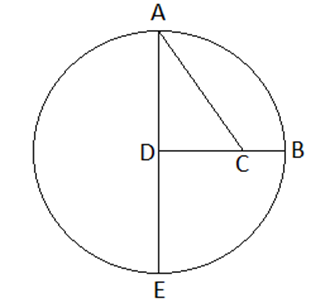
\includegraphics{24}

Note: Figure is not drawn to scale

\bigskip
In the figure above, circle $D$ has a circumference of $16\pi$ meters. If $BC=2$, what is the length of $AC$?

\begin{enumerate}[label=(\Alph*)]
\item 8
\item 10
\item 12
\item 16
\item $8\pi$
\end{enumerate}
}{\advanced

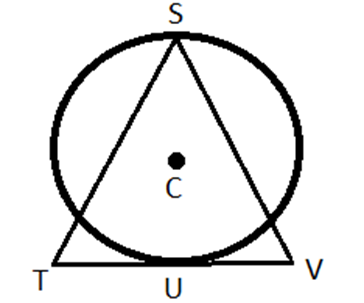
\includegraphics{25}

In the figure above, $SVT$ is an equilateral triangle and $TU=UV$. If the area of the circle is $9\pi$, what is the length of $ST$?

\begin{enumerate}[label=(\Alph*)]
\item $\sqrt{48}$
\item $\sqrt{40}$
\item $\sqrt{51}$
\item $\sqrt{45}$
\item $2\sqrt{11}$
\end{enumerate}}
\end{multienumerate}

\newpage
\section{Volume and Surface Area}

Examples:

\begin{multienumerate}
\mitemxx{\basic

9 small cubes with length 1 are combined to make one large shape. What is the minimum surface area of this larger shape?}
{\medium

The dimensions of an empty rectangular box $A$ are 8 inches by 8 inches by 5 inches. Box $B$ is a solid rectangular box with dimensions 4 inches by 4 inches by $1/3$ inches. What is the maximum number of boxes with the shape of box $B$ that could fit completely into Box $A$?

\begin{enumerate}[label=(\Alph*)]
\item 16
\item 24
\item 60
\item 90
\item 96
\end{enumerate}}
\end{multienumerate}

\hrulefill

\bigskip
Volume - volume is the area of the 2D figure and then multiply it by the height. For example, the volume of a cylinder is the area of a \longline multiplied by the \longline.

\vfill
Surface area - find the area of each side and then take the sum.

\begin{itemize}
\item Draw a cube and then write the formula for the surface area of a cube
\vfill\item Draw a rectangular prism and then write the formula for the surface area of a prism
\vfill\item Draw a cylinder and then write the formula for the surface area of a cylinder
\end{itemize}

\vfill
\pagebreak
\subsection{SAT Worksheet 4B: 6 Questions, 8 Minutes}

\begin{multienumerate}
\mitemxx{\basic

A sphere with a diameter $d$ is inscribed in a cube so that a total of 6 points on the sphere touch the cube. What is the area of the cube?

\begin{enumerate}[label=(\Alph*)]
\item $d^2$
\item $d^3$
\item $(1/8)d^3$
\item $6d$
\item $6d^3$
\end{enumerate}
}{\basic

A rectangular prism has a length of 6 square inches, a width of 6 square inches, and a height of 3 square inches. What is the minimum number of  square feet of wrapping paper would it take to wrap the entire shape?

\begin{enumerate}[label=(\Alph*)]
\item 0.333
\item 0.375
\item 1.0
\item 1.25
\item 108
\end{enumerate}}

\vfill
\mitemxx{\medium

\centerline{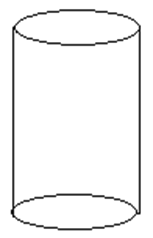
\includegraphics{26}}

Three tennis balls each with a diameter of 4 are placed in a canister of diameter 4 and height 12. Given that the area of a sphere is $4/3\pi r^3$, what is the remaining volume inside of the canister?

\begin{enumerate}[label=(\Alph*)]
\item $48\pi-(16/3)\pi$
\item $48\pi$
\item $24\pi-(8/3)\pi$
\item $24\pi-(16/3)\pi$
\item $48\pi-(112/3)\pi$
\end{enumerate}}{\medium

A rectangular prism with length 3, width 4, and height 7 has volume $v$. What is the volume of a rectangular prism with length 6, width 7, and height 1 in terms of $v$?

\begin{enumerate}[label=(\Alph*)]
\item $v$
\item $2v$
\item $v/4$
\item $42$
\item $v/2$
\end{enumerate}}

\vfill
\mitemxx{\advanced

A cylindrical water tank of height 10 square feet and a diameter of 10 square feet is filled with $\pi$ square inches of water every minute. How long would it take to fill 75\% of the water tank, in minutes?

\begin{enumerate}[label=(\Alph*)]
\item $75$
\item $62.5\pi$
\item $250/3$
\item $187.5$
\item $250\pi$
\end{enumerate}}{\advanced

A rectangular cylinder has a radius of $s$ and height $s$. What is the volume of the smallest cube that could be used to enclose this cylinder, in terms of $s$?

\begin{enumerate}[label=(\Alph*)]
\item $s^3/8$
\item $2s^3$
\item $s^3$
\item $8s^3$
\item $s^2$
\end{enumerate}}
\end{multienumerate}

\pagebreak
\subsection{SAT Worksheet 5B (Basic): 6 Questions, 8 Minutes}

\begin{multienumerate}
\mitemxx{1.  The area of square $A$ is $n$ and square $B$ has a side length that is twice that of square $A$. Which expression represents the area of square $B$?

\begin{enumerate}[label=(\Alph*)]
\item $n$
\item $n^2$
\item $n^4$
\item $2n$
\item $4n$
\end{enumerate}}{For which given value for the radius of a circle is the area greater in value than the circumference?

\begin{enumerate}[label=(\Alph*)]
\item 0.5
\item 1
\item 1.5
\item 2
\item 2.5
\end{enumerate}}

\vfill
\mitemxx{

\centerline{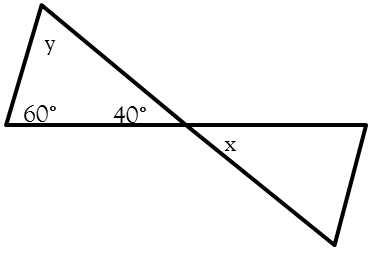
\includegraphics{27}}

In the figure above, what is the value of $x+y$?

\begin{enumerate}[label=(\Alph*)]
\item $70^\circ$
\item $80^\circ$
\item $100^\circ$
\item $120^\circ$
\item $140^\circ$
\end{enumerate}}{

\centerline{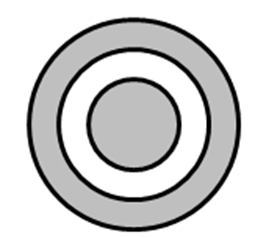
\includegraphics{28}}

In the figure above, the area of the inner most concentric circle is $9\pi$ cm. If each subsequent circle increases in radius by 1, what is the area of the outermost circle?

\begin{enumerate}[label=(\Alph*)]
\item $25\pi$
\item $36\pi$
\item $49\pi$
\item $121\pi$
\item $169\pi$
\end{enumerate}}

\vfill
\mitemxx{The total sum of the interior angles of a regular pentagon is $6m$. What is the measure of one angle?

\begin{enumerate}[label=(\Alph*)]
\item $m$
\item $5m$
\item $6m$
\item $(5/6)m$
\item $(6/5)m$
\end{enumerate}}{If the length of the diagonal of a square doubles, what ratio is the original side length to the new one?

\begin{enumerate}[label=(\Alph*)]
\item $1:2$
\item $1:4$
\item $2:1$
\item $4:1$
\item $1:\sqrt{2}$
\end{enumerate}}
\end{multienumerate}

\newpage
\textbf{\large SAT Worksheet 6B (Medium): 6 Questions, 9 Minutes}

\begin{multienumerate}
\mitemxx{

\medskip
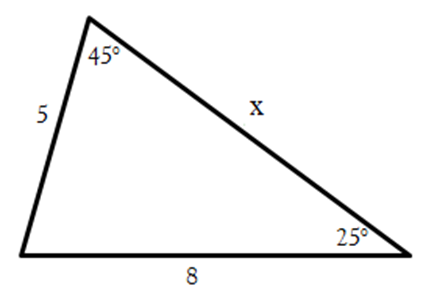
\includegraphics{29}

Which of the following could be a possible value of $x$ in the figure above?

\begin{enumerate}[label=(\Alph*)]
\item 3
\item 6
\item 7
\item 11
\item 13
\end{enumerate}}{

\medskip
\centerline{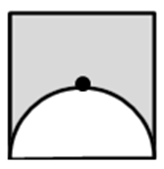
\includegraphics{30}}

Determine the area of the shaded region to the nearest hundredth in the figure above if the radius of the circle is 3.}

\vfill
\mitemxx{A 13 ft. ladder is propped against a building. If the top of the ladder reaches a height of 12 ft. on the building, what is the distance of base of the ladder to the base of the building in feet?

\begin{enumerate}[label=(\Alph*)]
\item 4
\item 5
\item 8
\item 11
\item 12
\end{enumerate}}{4. The surface area of a cube is equal to its volume. What is the length of the sides?

\begin{enumerate}[label=(\Alph*)]
\item 2 units
\item 4 units
\item 6 units
\item 8 units
\item 16 units
\end{enumerate}}

\vfill
\mitemxx{Find the measure of the radius of a right cylinder whose volume is twice the value of the height to the nearest hundredth.}{The volume of a ball is given by kπ where k is a positive integer. Which of the following is the smallest possible value of the volume? (The volume of a sphere is $4/3\pi r^3$.)

\begin{multicols}{2}
\begin{enumerate}[label=(\Alph*)]
\item $9\pi$
\item $12\pi$
\item $16\pi$
\item $36\pi$
\item $54\pi$
\end{enumerate}
\end{multicols}}
\end{multienumerate}

\pagebreak
\subsection{SAT Worksheet 7B (Advanced): 6 Questions, 10 Minutes}

\begin{multienumerate}
\mitemxx{If the area of an equilateral triangle is doubled, what is the ratio of the old side length to the new one?

\begin{enumerate}[label=(\Alph*)]
\item $1:\sqrt{2}$
\item $1:\sqrt{3}$
\item $1:2$
\item $1:3$
\item $2:\sqrt{3}$
\end{enumerate}}{In the figure below, the area of the inner circle is $6\pi$ and each outer circle has a width of 1 cm. greater than the previous circle. Determine the ratio of the radius of the outermost circle to the inner most.

\centerline{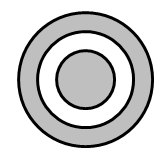
\includegraphics{31}}

\begin{enumerate}[label=(\Alph*)]
\item $6+4\sqrt{6}:6$
\item $6+2\sqrt{6}:6$
\item $2:3$
\item $3:4$
\item $1:3$
\end{enumerate}}

\vfill
\mitemxx{The area of a rectangle is equal to its perimeter. If the sum of the length and the width is 9, what is the length of the diagonal?

\begin{enumerate}[label=(\Alph*)]
\item $\sqrt{5}$
\item $3\sqrt{5}$
\item $2\sqrt{5}$
\item $3\sqrt{2}$
\item $5\sqrt{2}$
\end{enumerate}}{A cube with an edge of 3 cm. consists of smaller $1\times1$ cm. cubes. If the outer faces of the cube were painted, what is the ratio of the outer faces to the total number of faces of each smaller cube?

\begin{enumerate}[label=(\Alph*)]
\item $1:3$
\item $1:6$
\item $1:2$
\item $2:3$
\item $1:4$
\end{enumerate}}

\vfill
\mitemxx{

\medskip
\centerline{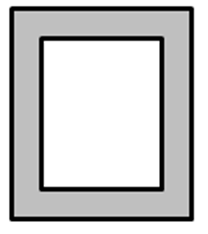
\includegraphics{32}}

A picture has a frame of uniform width. The dimensions of the frame are 12 cm and 8 cm. If the area of the picture is 32 cm$^2$, which of the following must be the width of the frame?

\begin{enumerate}[label=(\Alph*)]
\item 2 cm
\item 3 cm
\item 4 cm
\item 5 cm
\item 6 cm
\end{enumerate}}{

\medskip
\centerline{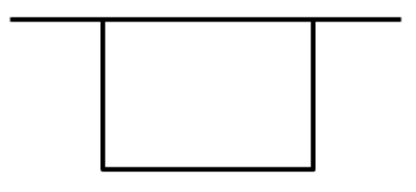
\includegraphics{33}}

Brandy wants to build a small fence around her rectangular garden that is adjacent to a wall. If she buys 40 feet of fencing, what is the maximum area of the garden she can cover?

\begin{enumerate}[label=(\Alph*)]
\item 10 ft$^2$
\item 24 ft$^2$
\item 100 ft$^2$
\item 200 ft$^2$
\item 400 ft$^2$
\end{enumerate}}
\end{multienumerate}